\section{Classification pipeline}

Internet is primary source of data
\begin{itemize}
\item Data sometimes questionable, misleading or erroneous
\item Actions take on basis of incorrect can have serious consequences
\end{itemize}

Performing a data analysis project is more than knowing and using a
classification algorithm. Main steps:
\begin{itemize}
\item Data collection and preparation (domain knowledge and
  understanding)
\item Model training, selection and assessment (understanding limits
  of machine learning is essential)
\end{itemize}

\subsection{Data collection and preparation}
\begin{itemize}
\item Feature identification
\item Labelling
\item Discretization
\item Feature selection
\item Feature normalization
\end{itemize}

\subsection{Model training}
\begin{itemize}
\item Selecting performance metrics
\item Model selection
\item Selecting training and test data
\end{itemize}

\subsection{Feature identification}
First step in collecting data. Definition of attributes (or features)
that describe a data item and the class label. Domain knowledge is
needed.

\subsubsection{Features}
Different types
\begin{itemize}
\item Numerical (age, temp, \ldots)
\item Ordinal (phone code, \ldots)
\item Categorical (student, weather, \ldots)
\end{itemize}

Some classifiers require categorical features $ \rightarrow $
discretization.

\subsubsection{Labelling}
Collecting lots of data is easy. Labelling is time consuming,
expensive, difficult and sometimes even impossible.

\textbf{How to obtain labels}
\begin{itemize}
\item Ask experts or DIY (expensive, boring, low volume)
\item Ask the crowd (less expensive, popular, unreliable)
\item Find some complementary info sources (distant learning)
\end{itemize}

\subsubsection{Crowdsourcing}
\begin{itemize}
\item Create a task to be done by crowd.
\item The task is submitted to crowdsourcing platform
\item Platform distributes task to interested workers that provide
  their answers and receive payment for it
\item Requester collects the answer
\end{itemize}

\subsubsection{Types of crowd-workers}
Truthful (expert or normal) \\
Untruthful (sloppy, uniform spammer, random spammer) \\
Leads to problem in aggregating answers.

\subsubsection{Non-iterative aggregation algorithms}

\subsubsection{Majority Decision (MD)}
\begin{itemize}
\item No pre-processing step
\item Estimate $ P(x_j = l ) $ as
  \begin{align*}
    & P(x_j = l) = \frac{1}{N} \sum_{i = 1}^N (1 \mid a_i (x_j) = l)
    \\
    & x_j \text{page to label} \\
    & N \text{number of workers} \\
    & l \text{label} \\
    & a_i(x_j) \text{answer of worker i on page } x_j
  \end{align*}
\end{itemize}

\subsubsection{Honey pot (HP)}
\begin{itemize}
\item Pre-processing step
  \begin{itemize}
  \item Insert pages $ x_1, x_2, \ldots, x_k$ for which labels are
    known $ l_1, l_2, \ldots, l_k $
  \item Remove workers and their answers that fail at correctly
    labelling more that m\% of pages (either spam or sloppy)
  \end{itemize}
\item Same decision rule as MD
\end{itemize}

\subsubsection{Iterative aggregation algorithms}
\subsubsection{Expectation maximization (EM)}
\begin{itemize}
\item E-Step: estimate the labels from the answers of the workers
\item M-Step: estimate the reliability of workers from the consistency
  of answers
\end{itemize}

\begin{itemize}
\item (E) step: estimate $ P(x_j = l ) $ as \\
  $ P(x_j = l) = \frac{1}{\sum_{i = 1}^N w_i} \sum_{i = 1}^N (w_i \mid
  a_i(x_j) = l) $
\item (M) step: update the expertise $ w_i $ as \\
  $ w_i = \frac{1}{M} \sum_{j = 1}^M (1 \mid a_i(x_j) = argmax_l P
  (x_j = l)) $ \\
  $ w_i $ expertise of worker i \\
  $ M $ number of items to label
\end{itemize}

\subsection{Discretization}

\subsubsection{Unsupervised discretization}
Equal witdh: divide range in predefined number of bin \\
Equal frequency: divide range in predefined number of bins so that
every bin contains the same number of values \\
Clustering: use any suitable clustering method for multi-dimensional
data and assign one feature value per cluster

\subsubsection{Supervised discretization}

Assuming a discretization is given. we may ask the question whether
the class labels depends on the interval. We can use $ \chi^2 $
statistics in order to test the independence of two adjacent
intervals.

\begin{table}[!htbp]
  \begin{tabular}{l|l|l|l}
    ~ & Class1 & Class2 & sum \\
    Interval 1 & $ O\_\{11\} = n\_\{11\} \$ \$ E\_\{11\} =\frac\{R1
                 \times C1\}\{N\} $  & $ O\_\{12\} = n\_\{12\} \$ \$
                                       E\_\{12\} = \frac\{R1 \times
                                       C2\}\{N\} $ & R1  \\ \hline

    Interval 2 & $ O\_\{21\} = n\_\{21\} $ $ E\_\{21\} = \frac\{R2
                 \times C1\}\{N\} $ & $ O\_\{22\} = n\_\{22\} $ $
                                      E\_\{22\} = \frac\{R2 \times
                                      C2\}\{N\} $ & R2 \\ \hline
    sum & C1 & C2 & N \\
  \end{tabular}
\end{table}

$ \chi^2 = \sum_{i=1,2} \sum_{i=1,2} \frac{(O_{ij} -
  E_{ij})^2}{E_{ij}} $ \\

If $ P(\chi^2 \mid DF = 1) > 0.05 $ merge the intervals, DF = degree
of freedom

\begin{itemize}
\item Can only be applied after unsupervised equal width
\item Attempts to merge intervals where class label does not depend on
  attribute value
\item Merges intervals if the value of $\chi^2$ is above 0.05
\item Works only for binary class labels
\end{itemize}

\subsection{Feature selection}

Reducing the number of N features to an optmial subset of M
features. There are $ \binom{N}{M} $ possible subsets.

\begin{itemize}
\item Filtering: consider features as independent
\item Wrapper: consider dependencies among features
\end{itemize}

\subsubsection{Filtering}
rank features according to their predictive power and select the best
ones. \textbf{Pros}:
\begin{itemize}
\item Independent of the classifier (performed only once)
\end{itemize}
\textbf{Cons}
\begin{itemize}
\item Independent of classifier (ignores interaction with classifier)
\item Assumes features are independent
\end{itemize}

\subsubsection{Ranking categorical features}
$ \chi^2 $ statistics: $ P(\chi^2 \mid DF = n - 1) $ gives a rank
measure. We perform an independence test between the feature values
and the class labels. \textbf{See above}.

\subsubsection{Ranking numerical features}
Mutual information between feature F and class label C
\begin{align*}
  I(F; C) & =  H(C) - H(C \mid F) = H(F) + H(C) - H(F, C) \\
  H(F) & = - \sum_i P(f_i)log_2 P(f_i) \\
  H(F, C) & = - \sum_i \sum_j P(f_i, c_j) log_2 P(f_i, c_j)
\end{align*}

Pitfalls:
\begin{itemize}
\item Correlation $ \neq $ causality
\item Collectively relevant features may look individually irrelevant
\end{itemize}

\subsubsection{Wrapping}
Iteratively add features
\begin{itemize}
\item at each iteration create a classifier and evaluate its
  performance
\item stop when no improvement
\end{itemize}
\textbf{Pros}
\begin{itemize}
\item interact with the classifier
\item no independence assumption
\end{itemize}

\textbf{Cons}
\begin{itemize}
\item Computationally expensive
\end{itemize}


\subsubsection{Feature normalization}
Some classifiers do not manage weel features with very different
scale. Feature with large values dominates the others and the
classifier over optimizes them.

\subsubsection{Standardisation and scaling}
\textbf{Standardisation}: map to normal distribution $ N(0, 1) $
\begin{itemize}
\item $ x'_i = \frac{x_i - \omega_i}{\sigma_i} $
\item $ \omega $ is the mean value of feature $ x_i $
\item $ \sigma_i $ is std dev
\item The new feature $ x'_i $ has mean 0 and std dev 1
\end{itemize}

\textbf{Scaling}: map to interval $ [0, 1] $
\begin{itemize}
\item $ x'_i = \frac{x_i - m_i}{M_i - m_i} $
\item $ M_i $ and $ m_i $ are the max and min  values of feature $ x_
  i $
\end{itemize}

\subsubsection{Standardisation vs.\ scaling}
Standardisation: assumes that data has been generated by guassian
process \\
Scaling: if data has outliets they scale the ``normal''' values to
very small interval

\subsection{Model training, selection and assessment}
Model assessment: having chosen a model, estimate the prediction error
no new data.

\subsubsection{Perf metric for binary classif}
For categorical binary classifications, the usual metrics consider
four types of outcomes. \\
Correct results:
\begin{itemize}
\item True positives
\item True negatives
\end{itemize}
Incorrect results
\begin{itemize}
\item False positive
\item False negatives
\end{itemize}

\subsubsection{Accuracy}

$ A = \frac{TP + TN} {TP + TN + FP + FN} = \frac{TP + TN}{N} $
Approriate when
\begin{itemize}
\item Classes are not skewed
\item Errors have same importance
\end{itemize}

Pitfalls
Skew:
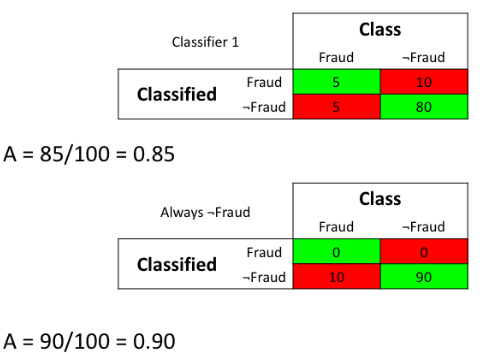
\includegraphics[width=200px, height=120px]{accpitskew}

\subsubsection{Precision and recall}
$ P = \frac{TP}{TP + FP} $ \\
$ R = \frac{TP}{TP + FN} $

\subsubsection{F-score}
$ F1 = 2 \cdot \frac{P \cdot R}{P + R} $ \\
$ F_\beta = \frac{(1 + \beta^2)P R}{(\beta^2 P + R)}$

\subsubsection{Considering cost}

Assign different importance to different outcomes:

\begin{table}[htp]
  \centering
  \caption{Cost assignation}
  \label{cost}
  \begin{tabular}{lll}
    & yes                & no                  \\
    yes & true positive: 30  & false negative: -30 \\
    no  & false positive: -1 & true negative: 1    \\
    &                    &
  \end{tabular}
\end{table}

\subsubsection{Model selection}
Parameters tuning:
\begin{itemize}
\item regularisation factor
\item threshold
\item distance function
\item number of neighbors
\end{itemize}

Estimate performance of different models to select best one.
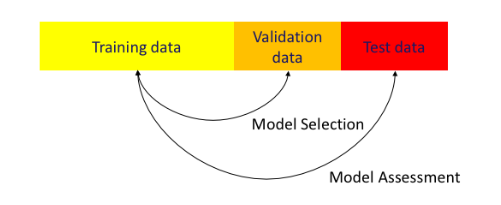
\includegraphics[height=120px, width=120px]{modass}
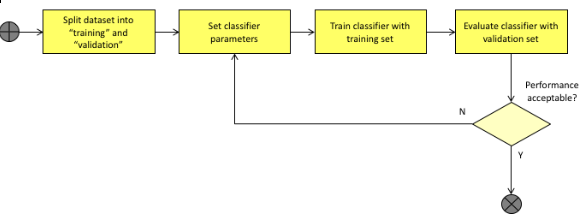
\includegraphics[height=100px, width=200px]{modsel}

\subsubsection{Loss function (error function)}
Categorical output:
\begin{itemize}
\item 0-1 loss function: $ J = \sum_{i=1}^n \#(y \neq f(x_i)) $
\end{itemize}
Real value output
\begin{itemize}
\item Squared error: $ J = \frac{1}{n} \sum_{i=1}^n (y_i - f(x_i))^2 $
\item Absolute error: $ J = \frac{1}{n}\sum_{i=1}^n \mid y_i - f(x_i)
  \mid $
\end{itemize}

\subsubsection{K-fold cross validation}

Split training set into k partitions, and train a model for each
subset. Then model is evaluated against the validation set minus the
partition it has been trained with. And performance averaged over all
k runs. Good compromise between unbiased estimate of true accuracy and
computation time.

\subsubsection{Leave one out cross validation}
Extreme form of k-fold. Each item is a partition. Most unbiased
estimate of true accuracy but time consuming because number of
iterations equals number of examples in dataset.

\subsubsection{Skewed distributions}
Some class labels might be heavily skewed, e.g.\:
\begin{itemize}
\item Non fake pages = 10000
\item Fake pages = 10
\end{itemize}
Rare data points not in validation set!

\subsubsection{Fighting skew}
Stratification:
\begin{itemize}
\item Select validation set as random sample but assure that each is
  class is approx.\ proportionaly represented
\end{itemize}
Over- and Under-sampling
\begin{itemize}
\item Including over-proportional number from the class
\item Include under-proportional number from larger class
\end{itemize}

\subsubsection{How good is a model?}
Model is function $ f_D $ that estimates a function: $ f: X^d
\rightarrow Y$ with $ y = f(X) $ \\
Evaluating error: \\
$ Err(f_D, T) = \frac{1}{\mid T \mid} \sum_{X \in T} (f_D(x) - y)^2 $
\begin{itemize}
\item D = Training set from which the model is learnt
\item T = Validation set on which error is evaluated
\item Squared error measure
\end{itemize}

\subsubsection{Training and test error}
\begin{itemize}
\item error on training set D: \textbf{training error} \\
  $ Err_{train} = Err(f_D, D) $
\item test on independent test set T: \textbf{test error} \\
  $ Err_{test} = Err(f_D, T) $
\end{itemize}

\subsubsection{Expected errors}
Repeatedly evaluate error for different models generated from
different training sets $ d \in D $.
\begin{itemize}
\item \textbf{Expected training error} \\
  $ EErr_{train} = E_D[Err(f_d, d)] = \frac{1}{\mid D \mid} \sum_{d
    \in D} Err(f_d, d) $
\item \textbf{Expected test error} \\
  $EErr_test = E_{D,T} [Err(f_d, T(d))] = \frac{1}{\mid D \mid \sum_{d
    \in D}} Err(f_d, T(d)) $
\end{itemize}

\subsubsection{Bias and variance}
The error can be rewritten as follows:
$ EErr_{test} = Bias^2 + Variance $ \\ where
\begin{itemize}
\item $ Bias = E_{D,T} [f_d(X) - y] $
\item $ Variance = E_{D, T} [(f_d(X) - \mathsf{f}(X))^2] $
\item $ \mathsf{f}(X) = E_{D}[f_d(x)] $
\end{itemize}

\subsubsection{Bias/Variance and model complexity}
There usually a bias variance tradeoff caused by model complexity
\begin{itemize}
\item Complex models usually have lower bias but higher variance:
  \textbf{overfitting}
\item Simple models have higher bias but lower variance:
  \textbf{under-fitting}
\end{itemize}

\subsection{Pitfalls}
\begin{itemize}
\item Beware of trusting correlations in a blind way
\item Beware of over-fitting, leads to bad prediction
\end{itemize}

\subsection{Does more data help}
Question: is more data better than a better algorithm?
Apparently all algorithms benefit very much from having more data, but
when looking in more details not so-clear cut.

%%% Local Variables:
%%% mode: latex
%%% TeX-master: "master"
%%% End:
